\section*{A3.1}

\subsection*{a)}
The predicate \texttt{writtenIn(M,T)} can be implemented as follows.

\begin{verbatim}
writtenIn(M,program(M)) :-
  program(M).

writtenIn(M,compiler(X, M, Y)) :-
  compiler(X, M, Y).

writtenIn(M,interpreter(X,M)) :-
  interpreter(X,M).
\end{verbatim}

The result of running \texttt{?-writtenIn(M,T)} is seen below.
\begin{figure}[h]
\centering
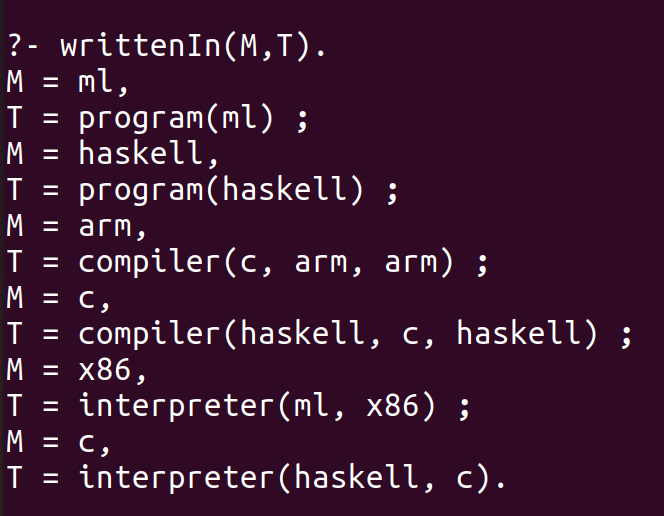
\includegraphics[width=0.5\textwidth]{a31a.png}
\caption{Result of running writtenIn.}
\end{figure}

\subsection*{b)}
The predicate \texttt{canRun(L)} could be implemented as follows.

\begin{verbatim}
canRun(L) :-
  machine(L).

canRun(L) :-
  interpreter(L,X),
  canRun(X).

canRun(L) :-
  compiler(L,X,Y),
  canRun(X),
  canRun(Y).
\end{verbatim}

The result of running \texttt{?-canRun(L)} is seen below.
\begin{figure}[h]
\centering
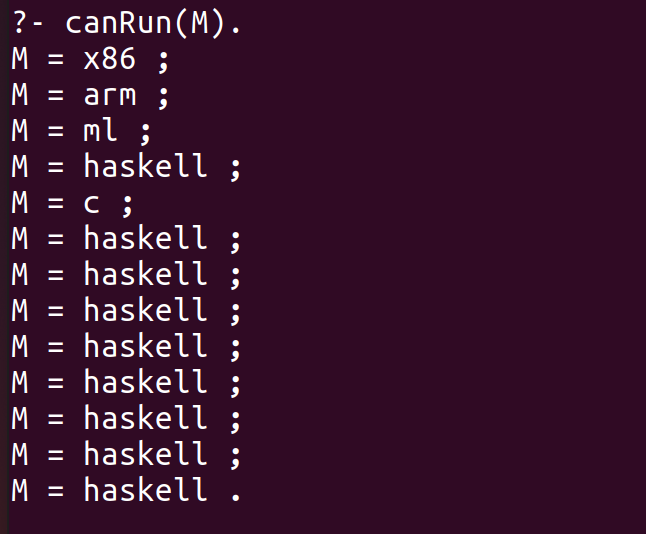
\includegraphics[width=0.5\textwidth]{a31b.png}
\caption{Result of running canRun.}
\end{figure}

\subsection*{c)}
To avoid getting \texttt{L = haskell} an infinite number of times, we add the condition that the compiler cannot translate the program into a new program in the same language. 

\begin{verbatim}
canRun(L) :-
  compiler(L,X,Y),
  L \= Y,
  canRun(X),
  canRun(Y).
\end{verbatim}

Now when running the query we get the following result.
\begin{figure}[h]
\centering
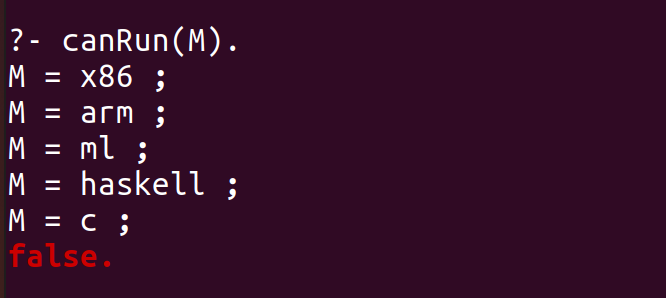
\includegraphics[width=0.5\textwidth]{a31c.png}
\caption{Result of running canRun.}
\end{figure}

